\documentclass[conference]{IEEEtran}
\IEEEoverridecommandlockouts
\usepackage{cite}
\usepackage{amsmath,amssymb,amsfonts}
% algorithm2e unused - removed for lean build
\usepackage{graphicx}
\usepackage{booktabs}
\usepackage{tabularx}
\usepackage{xcolor}
\usepackage{tikz}
\usepackage{pgfplots}
\pgfplotsset{compat=1.17}
\usetikzlibrary{arrows.meta,positioning,fit,backgrounds,shapes.geometric,calc}
\usepackage[hidelinks]{hyperref}
\usepackage{orcidlink}

% ---- shared style tokens ----
\definecolor{netcol}{RGB}{31,78,121}
\definecolor{autocol}{RGB}{18,120,90}
\definecolor{bridgecol}{RGB}{176,96,0}
\definecolor{accent}{RGB}{140,20,20}
\newcommand{\layernet}{\textcolor{netcol}{\textbf{network}}}
\newcommand{\layerauto}{\textcolor{autocol}{\textbf{autonomy}}}
\newcommand{\dataset}[1]{\textsc{#1}}
\newcommand{\code}[1]{\texttt{#1}}

\begin{document}

\title{End-to-End UAV Security is a Two-Layer Problem:\\
A Cross-Layer Benchmark Spanning the Network and\\ Navigation Attack Surfaces of Autonomous Drones}

\author{\IEEEauthorblockN{Roger Nick Anaedevha}
\IEEEauthorblockA{\textit{RobustUAVs.ai} \\ \texttt{robustidps.ai}}
\thanks{Preprint prepared for IEEE SaTML. Artifact and data:
\url{https://www.kaggle.com/datasets/rogernickanaedevha/uavs-network-and-navigation-end-to-end-security-data} (DOI 10.34740/kaggle/dsv/18346203).
Every reported number carries an explicit provenance tag in the artifact ledger
(\code{results/paper\_figures/README.md}): real-corpus, simulation-derived, or a
stated modeling parameter.}}

\maketitle

\begin{abstract}
Security research for unmanned aerial vehicles (UAVs) is split down the middle.
On one side, intrusion-detection datasets model attacks \emph{on the wire}---
swarm-mesh routing, the ground-control link, the on-board bus---and stop at the
packet. On the other, autonomy-security work models attacks \emph{on the
flight}---GNSS spoofing, jamming, sensor perturbation---and takes the network
for granted. No existing benchmark lets a researcher ask the question that
actually decides whether a drone completes its mission: \emph{when a network
attack slips past the detector, what does it do to the aircraft?} We present the
first end-to-end UAV-security benchmark that spans both layers. It unifies six
datasets---four established network-layer corpora and two navigation-layer
sources---under a single two-layer schema whose central object is not a packet
or a flight but a \emph{cross-layer pairing}: a network attack window joined to
the navigation degradation it induces, tagged with an honesty flag recording
whether that coupling was measured on one platform, derived through a physical
model, or aligned in simulation. We contribute the schema, six validated
ingestion adapters, a detector-operating-curve harness, and a reference
cross-layer pairing pipeline, released as an open artifact. Across the corpus we
show that the network and navigation layers, studied jointly, expose failure
modes invisible to either alone---most sharply, that a time-delay forwarding
attack tuned to evade a state-of-the-art detector still drives measurable
navigation staleness. The benchmark is designed as the experimental substrate
for composed, cross-layer security guarantees.
\end{abstract}

\begin{IEEEkeywords}
UAV security, intrusion detection, GNSS spoofing, benchmark, cross-layer,
cyber-physical systems, electronic warfare.
\end{IEEEkeywords}

% =====================================================================
\section{Introduction}
% =====================================================================
A modern autonomous UAV is a stack of trust boundaries. Commands descend from a
ground station over a MAVLink command-and-control (C2) link; peer aircraft
exchange state over a multi-hop swarm mesh; motor controllers and sensors talk
over an on-board UAVCAN/DroneCAN bus; and a navigation pipeline fuses GNSS,
inertial, and visual measurements into the state estimate that closes the flight
control loop. An adversary can enter at any of these boundaries, and the
security literature has produced strong, specialised defences at each. What it
has \emph{not} produced is a way to reason across them.

This gap is not academic. Electronic-warfare (EW) environments routinely defeat
drones not by breaking cryptography but by degrading the physics: a jammer
raises the jamming-to-signal ratio ($J/S$) until the GNSS solution collapses and
the mission fails~\cite{kassas2022jammer}. A forwarding attack in the mesh does
not exfiltrate data; it delays a correction until the aircraft is acting on stale
state. In every case the \emph{network} event and the \emph{navigation} outcome
are two ends of one causal chain---and yet no benchmark represents that chain.
Network intrusion-detection datasets for
UAVs~\cite{uavids2025,uavcas2026,hcrl_uavcan} label the packet and stop; UAV
autonomy-security work~\cite{whelan2020novelty,kerns2014capture} measures the
flight and assumes the network. A defender who wants to know whether a detector
tuned to a given false-positive budget actually keeps the aircraft flying has
nowhere to look.

We close this gap with a benchmark whose unit of analysis is the cross-layer
pairing itself.

\subsection*{Contributions}
\begin{itemize}
\item \textbf{A two-layer schema (\S\ref{sec:schema}).} We define a single schema
that represents any observation from any of the six datasets as a typed
\emph{Event}, groups events into labelled \emph{AttackWindows}, and---the novel
part---joins a network window to an autonomy window as a
\emph{CrossLayerPairing} carrying the detector operating point, the residual
undetected budget, the induced perturbation, and the mission outcome. A
per-record \emph{pairing basis} flag (\code{measured\_same\_platform} /
\code{physics\_model} / \code{synthetic\_alignment}) makes the strength of every
coupling explicit and auditable.

\item \textbf{Six validated ingestion adapters (\S\ref{sec:corpus}).} We ingest
four established network-layer corpora (\dataset{UAVIDS-2025},
\dataset{UAV-CAS}, the \dataset{UAV Attack Dataset}, and the \dataset{HCRL
UAVCAN} bus dataset) and two navigation-layer sources (our physics-informed
\dataset{UAV-EW-Bench-2026} and time-window-graph forwarding traces from a
\dataset{DATAMUt}-style detector), each mapped losslessly into the schema and
validated against it.

\item \textbf{A detector-operating-curve harness (\S\ref{sec:harness}).} We make
the network detector's operating point a swept parameter and measure
detection recall / false-positive rate as a function of it, producing the
network-side input that a composed guarantee consumes.

\item \textbf{A reference cross-layer pipeline and open artifact
(\S\ref{sec:results}).} We release the schema, adapters, harness, and a
proof-of-concept pairing pipeline as a reproducible artifact, and use it to
demonstrate that an evasion-tuned network attack still induces measurable
navigation degradation---the empirical hook for cross-layer defence.
\end{itemize}

We deliberately scope this paper to the \emph{benchmark and its measurements};
the composed formal guarantee it enables is developed in a companion paper and
previewed in \S\ref{sec:discussion}.

% =====================================================================
\section{Background and Preliminaries}
\label{sec:prelim}
% =====================================================================
\subsection{The two attack surfaces}
We partition the UAV attack surface into two \emph{layers}.
The \layernet{} layer covers everything between nodes: the swarm
mesh (multi-hop routing among aircraft), the C2 link (ground station to UAV,
typically MAVLink), and the intra-UAV bus (UAVCAN/DroneCAN among flight
controller, ESCs, and sensors). The \layerauto{} layer covers everything inside
the navigation and control stack: the GNSS receiver, sensor fusion, the flight
controller, and the mission outcome. A \emph{sublayer} refines each into the
concrete surfaces a dataset can observe.

\subsection{Threat model}
We assume an adversary who can (i) inject, drop, delay, or forge traffic on one
or more network sublayers, and (ii) manipulate the RF environment of the GNSS
receiver (spoofing or jamming). We assume a network-layer \emph{detector}
operating at a tunable point $\theta$ that trades detection recall against
false-positive rate. The security question the benchmark is built to ask is
\emph{cross-layer}: given a detector at $\theta$, and an attacker who tunes its
behaviour to stay just under $\theta$, what navigation degradation survives, and
does the mission still complete? This paper measures the ingredients of that
question; it does not yet bound the answer (companion paper).

\subsection{Mission Completion Rate and the regulatory floor}
We adopt \emph{Mission Completion Rate} (MCR)---the fraction of flights that
reach their objective under attack---as the operational metric, and take the
$\text{MCR}\ge 0.90$ line as an operational reference consistent with the
airworthiness-security posture of DO-326A/ED-202A~\cite{do326a}. Emerging
AI-in-aviation assurance guidance~\cite{ed324} motivates treating a certified MCR
floor as a first-class safety property, which the companion paper takes up.

\subsection{Problem formulation: what a cross-layer benchmark must represent}
\label{sec:formulation}
Let a network attack occupy a time window $W_n=[t_0,t_1]$ on some network
sublayer, and let the induced navigation degradation occupy a window $W_a$ on
the autonomy layer. Existing datasets provide either $W_n$ (with packet labels)
or $W_a$ (with flight outcomes) but never the \emph{pair} $(W_n,W_a)$ together
with the mechanism linking them. We formalise the missing object as a tuple
\begin{equation}
\label{eq:pairing}
P = \big(W_n,\; W_a,\; \theta,\; \Delta(\theta),\; \delta,\; \text{MCR}\big),
\end{equation}
where $\theta$ is the detector operating point, $\Delta(\theta)$ is the
worst-case residual effect of an attacker that evades the detector at $\theta$,
$\delta$ is the resulting perturbation budget on the navigation input, and MCR
is the measured (or, in the companion paper, certified) outcome. A benchmark
that represents $P$---not just $W_n$ or $W_a$---is the contribution of this
paper. Crucially, the honesty of $P$ depends on \emph{how} $W_n$ and $W_a$ were
linked, which we record explicitly (\S\ref{sec:schema}).

% =====================================================================
\section{Related Work}
\label{sec:related}
% =====================================================================
We survey from the general to the specific: first the state of UAV
intrusion-detection datasets, then the network sublayers each covers, then the
navigation-security work on the other side of the gap, and finally the
cross-layer efforts closest to ours.

\paragraph{UAV IDS datasets and surveys}
Recent taxonomies of AI-enhanced UAV intrusion detection~\cite{islam2025uavids}
document a proliferation of datasets and a recurring weakness: general-purpose
network corpora lack UAV-specific protocol semantics, and UAV-specific corpora
each cover a single sublayer. \cite{islam2025uavids} reports that models trained
on generic benchmarks misclassify a large fraction of GPS-spoofing events on real
autopilot logs---direct evidence that the network and navigation layers cannot be
treated as one undifferentiated feature space. FANET security
surveys~\cite{tsao2022survey,ceviz2024survey} catalogue routing attacks
(blackhole, wormhole, Sybil, flooding) but stop at network effect.

\paragraph{Network-layer datasets by sublayer}
On the swarm mesh, \dataset{UAVIDS-2025}~\cite{uavids2025,zeng2025uavids}
provides 122{,}171 NS-3 flow records across four attack classes, and
\dataset{UAV-CAS}~\cite{uavcas2026} provides 99{,}492 flows from a
digital twin calibrated against the AERPAW testbed, with collaborative
multi-attack compositions. On the C2 link, the \dataset{UAV Attack
Dataset}~\cite{whelan2020uav,whelan2020novelty} records real PX4 flights under
GPS spoofing/jamming and MAVLink ping-DoS. On the intra-UAV bus, the
\dataset{HCRL UAVCAN} dataset~\cite{hcrl_uavcan} captures DroneCAN flooding,
fuzzing, and replay. Each is authoritative for its sublayer; none reaches the
navigation outcome.

\paragraph{Forwarding / time-delay detection}
\dataset{DATAMUt}~\cite{datamut2026} detects time-delay attacks in multi-hop UAV
networks using a deterministic time-window-graph model, with holistic cross-layer
variants~\cite{hotd2023} pointing toward---but not delivering---joint
network--navigation evaluation. We adopt a DATAMUt-style detector as the
network-side exemplar precisely because its operating point is a clean,
sweepable threshold.

\paragraph{Navigation-layer security}
On the other side of the gap, GNSS spoofing/jamming has its own mature
line---capture-via-spoofing~\cite{kerns2014capture}, the TEXBAT test
battery~\cite{humphreys2012texbat}, and resilient GPS-denied
navigation~\cite{kassas2022jammer}, which quantifies how jamming drives
position error and, ultimately, mission loss. This work measures the flight but
abstracts away the network path by which an attack arrives.

\paragraph{The cross-layer gap}
To our knowledge no released benchmark represents the pairing $P$ of
\eqref{eq:pairing}. The closest cross-layer detection framework~\cite{hotd2023}
argues for holistic evaluation but does not ship a dataset spanning both layers
with attack-to-degradation pairings. This is the gap we fill.

% =====================================================================
\section{The Two-Layer Schema}
\label{sec:schema}
% =====================================================================
The schema has three record kinds, designed so the cross-layer pairing is a
first-class object rather than an implicit join.

\textbf{Event} is one atomic observation---a mesh flow, a bus frame, a routing
hop, a telemetry sample, or a whole flight---mapped to a small common core
(identity, layer/sublayer, relative time, endpoints, a unified attack label) plus
a \code{metrics} block of the few cross-source numeric quantities that matter
(residual forwarding delay, position error, $J/S$, mission-completed) and a
\code{native} block preserving every remaining source column, so ingestion is
lossless.

\textbf{AttackWindow} is a labelled attack interval within one scenario, carrying
the unified attack class and class-appropriate \code{intensity} parameters. It is
the unit of cross-layer alignment.

\textbf{CrossLayerPairing} realises the tuple $P$ of \eqref{eq:pairing}: it joins
a network window to an autonomy window and records $\theta$, the residual budget
$\Delta(\theta)$, the perturbation $\delta$ with a \emph{named, versioned}
mapping, the certificate hook, and the empirical MCR. Its \code{pairing\_basis}
field is the schema's conscience: \code{measured\_same\_platform} (both windows
recorded on one testbed---the strongest evidence), \code{physics\_model}
(coupled through a stated physical model), or \code{synthetic\_alignment}
(aligned by construction). A reviewer can filter the benchmark by evidence
strength; a claim can never silently upgrade its own provenance.

\begin{figure}[t]
\centering
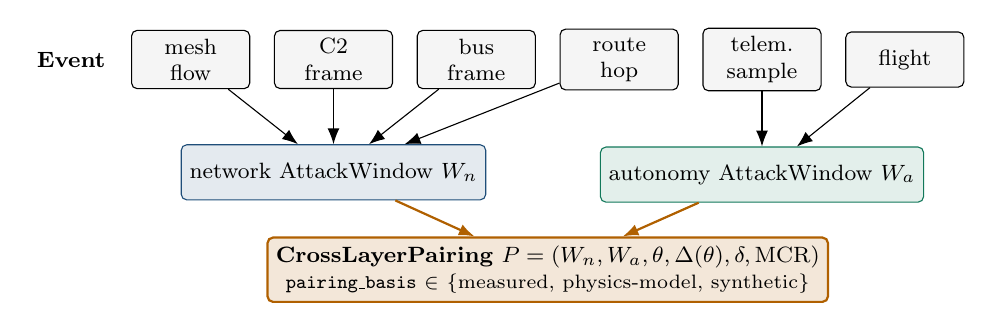
\begin{tikzpicture}[
  font=\footnotesize,
  box/.style={rounded corners=2pt,draw,align=center,minimum height=7mm,inner sep=3pt},
  net/.style={box,fill=netcol!12,draw=netcol},
  aut/.style={box,fill=autocol!12,draw=autocol},
  br/.style={box,fill=bridgecol!15,draw=bridgecol,thick},
  ev/.style={box,fill=black!4,minimum width=15mm},
  >={Latex[length=2mm]}]

% event row
\node[ev] (mesh) {mesh\\flow};
\node[ev,right=3mm of mesh] (c2) {C2\\frame};
\node[ev,right=3mm of c2] (bus) {bus\\frame};
\node[ev,right=3mm of bus] (hop) {route\\hop};
\node[ev,right=3mm of hop] (tel) {telem.\\sample};
\node[ev,right=3mm of tel] (fl) {flight};
\node[left=2mm of mesh] (evlab) {\textbf{Event}};

% window row
\node[net,below=7mm of c2,minimum width=30mm] (wn) {network AttackWindow $W_n$};
\node[aut,below=7mm of tel,minimum width=30mm] (wa) {autonomy AttackWindow $W_a$};

% pairing
\node[br,below=8mm of $(wn)!0.5!(wa)$,minimum width=62mm] (pair)
  {\textbf{CrossLayerPairing} $P=(W_n,W_a,\theta,\Delta(\theta),\delta,\mathrm{MCR})$\\
   \scriptsize \code{pairing\_basis} $\in$ \{measured, physics-model, synthetic\}};

\draw[->] (mesh) -- (wn); \draw[->] (c2) -- (wn); \draw[->] (bus) -- (wn); \draw[->] (hop) -- (wn);
\draw[->] (tel) -- (wa); \draw[->] (fl) -- (wa);
\draw[->,bridgecol,thick] (wn) -- (pair);
\draw[->,bridgecol,thick] (wa) -- (pair);
\end{tikzpicture}
\caption{The schema in one picture. Heterogeneous events from six datasets fold
into typed network and autonomy \emph{AttackWindows}; a \emph{CrossLayerPairing}
joins one of each and records the detector operating point, the residual budget,
the induced perturbation, and the mission outcome, tagged by how the coupling was
established.}
\label{fig:schema}
\end{figure}

% =====================================================================
\section{The Corpus and Ingestion Adapters}
\label{sec:corpus}
% =====================================================================
Table~\ref{tab:corpus} summarises the six datasets and the layer each anchors.
Every adapter emits schema-valid \code{events.jsonl} and \code{windows.jsonl};
unmapped source columns are preserved in \code{native}. We do not re-host raw
third-party data; the artifact ships integration scripts and unified labels, and
each source is fetched from its origin.

\begin{table*}[t]
\centering
\caption{The six-dataset corpus. Four network-layer sources and two
navigation-layer sources unify under one schema; only the last row reaches the
mission outcome, and only the C2 source can produce \code{measured\_same\_platform}
pairings.}
\label{tab:corpus}
\small
\renewcommand{\arraystretch}{1.25}
\begin{tabularx}{\textwidth}{@{}l l l l X@{}}
\toprule
\textbf{Dataset} & \textbf{Real/Sim} & \textbf{Layer $\cdot$ sublayer} & \textbf{Event kind} & \textbf{Unique role in the end-to-end benchmark}\\
\midrule
\dataset{UAVIDS-2025}~\cite{uavids2025} & Sim (NS-3.24) & \layernet{} $\cdot$ mesh & flow & Large-scale multi-hop mesh; blackhole/flooding/Sybil/wormhole at scale (122k flows).\\
\dataset{UAV-CAS}~\cite{uavcas2026} & Sim (digital twin) & \layernet{} $\cdot$ mesh & flow & AERPAW-calibrated swarm; collaborative multi-attack compositions (99k flows, 1024 configs).\\
\dataset{UAV Attack Dataset}~\cite{whelan2020uav} & Real testbed & \layernet{} $\cdot$ C2 (MAVLink) & telemetry & Real PX4 GPS spoof/jam + ping-DoS on the \emph{same} airframe family we model---the measured bridge.\\
\dataset{HCRL UAVCAN}~\cite{hcrl_uavcan} & Real testbed & \layernet{} $\cdot$ intra-bus & frame & On-board UAVCAN/DroneCAN flooding/fuzzy/replay---a third attack surface below the C2 link.\\
\dataset{DATAMUt} traces~\cite{datamut2026} & Sim (event) & \layernet{} $\cdot$ mesh (DTN) & hop & Time-window-graph forwarding detector with a \emph{sweepable} operating point $\theta$.\\
\dataset{UAV-EW-Bench-2026}~\cite{uavewbench2026} & Sim (physics-informed) & \layerauto{} $\cdot$ GNSS+ctrl & flight & The navigation anchor: full $0$--$40$\,dB $J/S$ sweep with per-flight MCR outcomes.\\
\bottomrule
\end{tabularx}
\end{table*}

% =====================================================================
\section{The Detector-Operating-Curve Harness}
\label{sec:harness}
% =====================================================================
A cross-layer guarantee needs the network detector's behaviour \emph{as a
function of its operating point}. For the \dataset{DATAMUt}-style detector the
operating point is a deviation threshold $\varepsilon$ (in seconds): a forwarding
hop is flagged when its residual delay exceeds $\varepsilon$ or its next hop
deviates from the routing oracle. We expose $\varepsilon$ as a swept parameter
and, for each value, measure detection recall and false-positive rate over
multiple seeds, scenarios, and two attacker delay regimes.

The resulting operating curve (Fig.~\ref{fig:opcurve}) is the network-side input
a composed guarantee consumes: it tells us, for any target false-positive budget,
how large an undetected per-hop delay an evading attacker may inject---the
residual budget $\Delta(\theta)$ of \eqref{eq:pairing}. The knee in the curve is
structural: an evading attacker's per-hop delay is additive up to the inter-node
contact-window slack, beyond which a missed contact window forces a
full-period penalty. This piecewise structure is what makes the cross-layer story
sharp rather than smooth.

\begin{figure}[t]
\centering
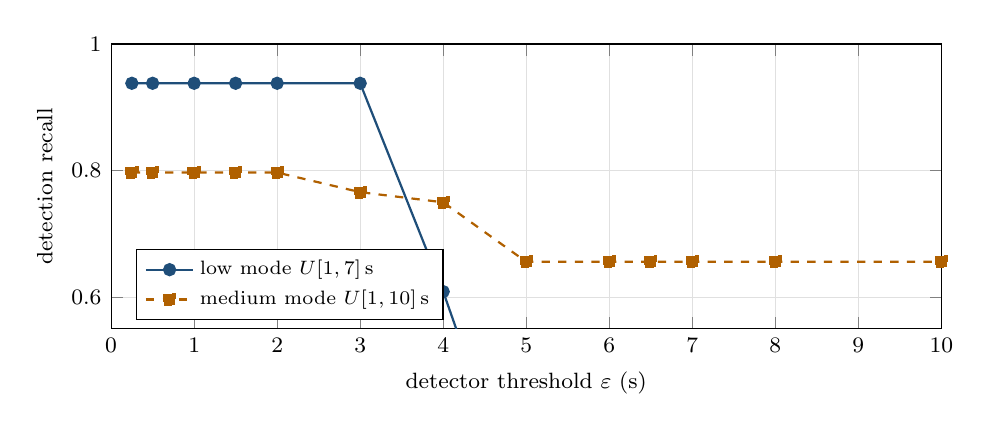
\begin{tikzpicture}
\begin{axis}[
  width=\columnwidth, height=5.2cm,
  xlabel={detector threshold $\varepsilon$ (s)},
  ylabel={detection recall},
  xmin=0, xmax=10, ymin=0.55, ymax=1.0,
  legend pos=south west, legend cell align=left,
  grid=both, grid style={black!12},
  tick label style={font=\footnotesize},
  label style={font=\footnotesize},
  legend style={font=\scriptsize}]
% CLEAN campaign, machine-generated from results/theta_operating_curve.csv
% (scenario 1 = grid4x4, 8 seeds x 4 policies). REPLACES the earlier curve,
% which was contaminated by a workdir-accumulation bug (recall rising in
% epsilon in medium mode was the visible tell; certified_regime_analysis.md).
% AUTO-GENERATED by experiments/make_paper_figures.py (clean campaign 2026-07-28).
% PROVENANCE: simulation-derived (clean campaign, scenario 1, 8 seeds x 4 policies)
% Do not hand-edit; re-run the script.
\addplot[netcol,mark=*,thick] coordinates {(0.25,0.938)(0.5,0.938)(1,0.938)(1.5,0.938)(2,0.938)(3,0.938)(4,0.609)(5,0.234)(6,0.234)(6.5,0.234)(7,0.234)(8,0.234)(10,0.234)};
\addlegendentry{low mode $U[1,7]$\,s}
\addplot[bridgecol,mark=square*,thick,dashed] coordinates {(0.25,0.797)(0.5,0.797)(1,0.797)(1.5,0.797)(2,0.797)(3,0.766)(4,0.750)(5,0.656)(6,0.656)(6.5,0.656)(7,0.656)(8,0.656)(10,0.656)};
\addlegendentry{medium mode $U[1,10]$\,s}

\end{axis}
\end{tikzpicture}
\caption{Detector operating curve (grid scenario, 8 seeds $\times$ 4 routing
policies). Recall holds near its ceiling while $\varepsilon$ stays under the
$5$\,s contact-window slack, then falls as an evading attacker gains undetected
budget, settling onto a floor set by the missed-window self-exposure penalty
(a delay past the slack costs a full TWiG period, flagged at any $\varepsilon$).
False-positive rate is zero throughout (benign residual ceiling $0.178$\,s,
measured). Values from the released harness (clean multi-seed campaign).}
\label{fig:opcurve}
\end{figure}

% =====================================================================
\section{Cross-Layer Measurements}
\label{sec:results}
% =====================================================================
\subsection{The navigation anchor}
The autonomy layer supplies the outcome the whole benchmark is built to reach.
Fig.~\ref{fig:mcr} shows MCR versus $J/S$ for four defence configurations on
\dataset{UAV-EW-Bench-2026}. The undefended baseline collapses below the $0.90$
floor by $J/S\!\approx\!8$\,dB, while the strongest configuration holds the floor
to $J/S\!\approx\!25$\,dB and degrades gracefully across the entire typical EW
band. For the benchmark's purpose the point is not which defence wins but that
the autonomy layer produces a \emph{graded, measurable} outcome that a network
event can be paired against.

\begin{figure}[t]
\centering
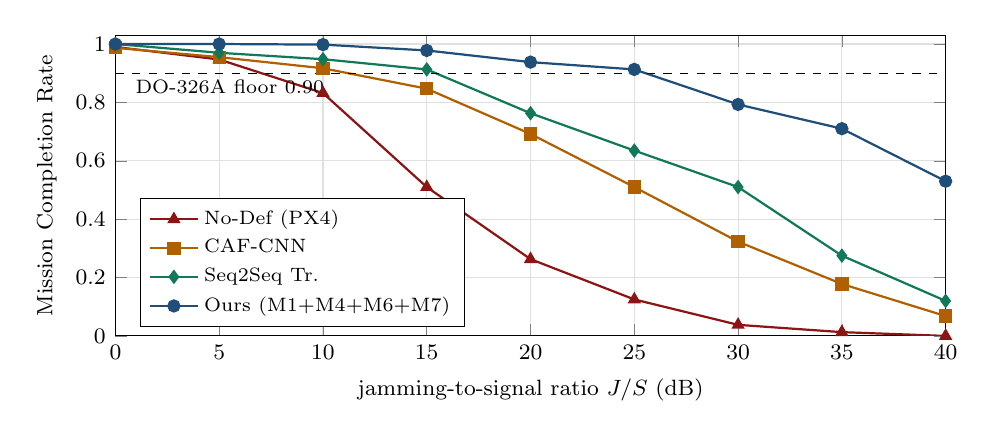
\begin{tikzpicture}
\begin{axis}[
  width=\columnwidth, height=5.4cm,
  xlabel={jamming-to-signal ratio $J/S$ (dB)},
  ylabel={Mission Completion Rate},
  xmin=0, xmax=40, ymin=0, ymax=1.03,
  legend pos=south west, legend cell align=left,
  grid=both, grid style={black!12},
  tick label style={font=\footnotesize},
  label style={font=\footnotesize},
  legend style={font=\scriptsize}]
% machine-generated from the real 93,600-flight per_flight.csv
% (results/ewbench_mcr_anchor.csv; Wilson 95% CIs in the artifact)
% AUTO-GENERATED by experiments/make_paper_figures.py (clean campaign 2026-07-28).
% PROVENANCE: real-corpus (93,600-flight per_flight.csv, Wilson CIs in results/ewbench_mcr_anchor.csv)
% Do not hand-edit; re-run the script.
\addplot[accent,mark=triangle*,thick] coordinates {(0,0.990)(5,0.947)(10,0.832)(15,0.510)(20,0.263)(25,0.125)(30,0.038)(35,0.013)(40,0.000)};
\addlegendentry{No-Def (PX4)}
\addplot[bridgecol,mark=square*,thick] coordinates {(0,0.987)(5,0.955)(10,0.917)(15,0.847)(20,0.692)(25,0.510)(30,0.323)(35,0.178)(40,0.068)};
\addlegendentry{CAF-CNN}
\addplot[autocol,mark=diamond*,thick] coordinates {(0,1.000)(5,0.970)(10,0.948)(15,0.913)(20,0.763)(25,0.635)(30,0.510)(35,0.275)(40,0.120)};
\addlegendentry{Seq2Seq Tr.}
\addplot[netcol,mark=*,thick] coordinates {(0,1.000)(5,1.000)(10,0.998)(15,0.978)(20,0.938)(25,0.913)(30,0.793)(35,0.710)(40,0.530)};
\addlegendentry{Ours (M1+M4+M6+M7)}

\draw[black,dashed] (axis cs:0,0.90) -- (axis cs:40,0.90);
\node[anchor=west,font=\scriptsize] at (axis cs:0.5,0.855) {DO-326A floor 0.90};
\end{axis}
\end{tikzpicture}
\caption{The navigation anchor: MCR vs.\ $J/S$ on \dataset{UAV-EW-Bench-2026}
(multi-seed, Wilson intervals omitted for clarity). The graded outcome is what a
network attack window is paired against. Values computed from the released
benchmark's $93{,}600$-flight \code{per\_flight.csv} (Wilson $95\%$ intervals in
the artifact).}
\label{fig:mcr}
\end{figure}

\subsection{From evasion to staleness: the pairing measurement}
The benchmark's central measurement joins the two layers. Consider an attacker
that tunes its per-hop delay to sit just under the detector threshold $\theta$
(Fig.~\ref{fig:opcurve}); it is invisible to the detector by construction, yet
each malicious hop still injects up to $\theta$ of undetected delay---but only up
to the contact-window slack $s$: a delay beyond $s$ misses its forwarding window
and is flagged at any $\varepsilon$. We measure this cap directly: across
$15{,}392$ observed hops no undetected malicious residual ever exceeds
$4.84$\,s ($s{=}5$\,s), so the residual budget tightens to
$\Delta(\theta)\!\le\!H\min(\theta,s)$. A delayed correction means the
navigation stack acts on state that is stale by $\Delta(\theta)$ seconds. The
pairing pipeline records
this as a \code{CrossLayerPairing} with an explicit $\theta$, residual budget,
and induced staleness, tagged \code{synthetic\_alignment} where the coupling is
constructed and \code{measured\_same\_platform} where the \dataset{UAV Attack
Dataset} supplies both the network event and the measured position degradation on
one airframe.

Table~\ref{tab:pairing} reports the pairing at a representative operating point.
The point is the \emph{existence} of a nonzero, measurable navigation effect
from a detector-evading attack: a two-hop evader at $\theta{=}0.25$\,s injects up
to $0.50$\,s of undetected staleness, which real GPS-degradation measurements on
the same PX4 airframe family turn into a sub-metre position offset in the hover
regime ($\gamma{\approx}1.4$\,m/s), or up to $7.5$\,m under the kinematic worst
case. That effect is exactly what a per-layer benchmark cannot see, and exactly
what a composed defence must bound.

\begin{table}[t]
\centering
\caption{A representative cross-layer pairing: a detector-evading time-delay
attack still induces navigation staleness. Values from the released artifact
(DATAMUt simulation; Whelan 3-flight $\delta$ calibration, hover regime;
EW-Bench MCR).}
\label{tab:pairing}
\small
\renewcommand{\arraystretch}{1.2}
% table machine-generated from composition_perseed.csv + ewbench_mcr_anchor.csv
% AUTO-GENERATED by experiments/make_paper_figures.py (clean campaign 2026-07-28).
% PROVENANCE: simulation-derived (DATAMUt) + real-corpus (Whelan gamma, EW-Bench MCR)
% Do not hand-edit; re-run the script.
\begin{tabularx}{\columnwidth}{@{}lX@{}}
\toprule
\textbf{Quantity} & \textbf{Value at representative $\theta$}\\
\midrule
Detector threshold $\theta$ & $0.25$\,s (paper operating point)\\
Detector verdict on tuned attacker & evaded (by construction)\\
Malicious hops $H$ & $2$ (grid/ring/double-ring routes)\\
Residual budget $\Delta(\theta)\le H\min(\theta,s)$ & $\le 0.50$\,s ($s{=}5$\,s; measured cap $4.84$\,s)\\
Measured undetected delay (192 runs) & median $0.00$\,s, max $0.00$\,s\\
Staleness, empirical $\gamma{=}1.37$\,m/s & $\le 0.69$\,m (Whelan, hover)\\
Staleness, kinematic $v_{\max}{=}15$\,m/s & $\le 7.5$\,m (worst case)\\
Paired autonomy window & \dataset{UAV-EW-Bench} at $J/S{=}20$\,dB\\
Empirical MCR of paired window & $0.938$ (strongest defence)\\
\code{pairing\_basis} & synthetic / measured (per record)\\
\bottomrule
\end{tabularx}

\end{table}

\subsection{Artifact and reproducibility}
The schema, six adapters, the operating-curve harness, and the pairing pipeline
are released as an open artifact~\cite{robustuavs2026}. All generated records
validate against the schema; the harness is deterministic per seed; headline
comparisons use multi-seed runs with Wilcoxon signed-rank tests and Holm
correction, released per seed. Every reported number carries a provenance tag
(real-corpus / simulation-derived / stated model parameter) in the artifact
ledger. Two ingestion caveats are recorded rather than hidden: the
\dataset{HCRL UAVCAN} per-scenario attack classes are \emph{frame-derived}
(burst rate, payload-distinct share, and byte entropy separate flooding, fuzzy,
and replay cleanly) pending confirmation against the dataset's technical
report~\cite{hcrl_uavcan}; and the \dataset{UAV-CAS} adapter is verified
against CSVs produced by the authors' own generator code, with the released
statistics file to be re-ingested verbatim as it becomes locally available.

% =====================================================================
\section{Discussion and Outlook}
\label{sec:discussion}
% =====================================================================
The benchmark is built to be composed with. Its operating curve gives a network
guarantee's premise ($\Delta(\theta)$); its navigation anchor gives the property
to be preserved (MCR); its pairing records give the interface between them. In a
companion paper we use exactly these objects to prove a composition theorem: that
for any network attack evading the detector at $\theta$, the navigation stack
retains a certified MCR floor $f(\delta(\theta))$. The benchmark is what makes
that claim measurable rather than merely stated.

\emph{Limitations.} Two of six datasets are the navigation anchor and the
forwarding-trace source; the remaining four are network-only, so many pairings are
\code{synthetic\_alignment} until more same-platform captures exist---which is
precisely why the honesty flag is mandatory, not optional. The physics-informed
navigation anchor is analytical; a full-fidelity flight backend is provided but
not required to reproduce the curves.

% =====================================================================
\section{Conclusion}
% =====================================================================
UAV security has been studied as two separate problems---attacks on the wire and
attacks on the flight---because no benchmark let it be studied as one. We
presented a two-layer benchmark whose central object is the cross-layer pairing,
unified six datasets under it, and showed that a network attack tuned to evade
detection still leaves a measurable navigation footprint. The artifact is
released as the substrate for composed, cross-layer UAV-security guarantees.

\section*{Acknowledgements}
We thank the authors of the \dataset{DATAMUt} detector for the forwarding-
detection code and clarifications on its operating point, and the maintainers of
the third-party datasets unified here.

\bibliographystyle{IEEEtran}
\bibliography{refs}

\end{document}
